\chapter{Ausarbeitung}
\section{Aufgabe 1}
\subsection{konstante Position}
\begin{gather}
	\frac{d}{dt}\begin{bmatrix}
	x \\
	y
	\end{bmatrix} = \begin{bmatrix}
	0 \\
	0
	\end{bmatrix} = \begin{bmatrix}
	0 & 0 \\
	0 & 0
	\end{bmatrix} \begin{bmatrix}
	x \\
	y
	\end{bmatrix}
\end{gather}
Übergangsmatrix:
\begin{gather}
	\bm{F} = \begin{bmatrix}
	0 & 0 \\
	0 & 0
	\end{bmatrix} \\
	\bm{\Phi}(\Delta t) = e^{\bm{F}\Delta t} =\begin{bmatrix}
	1 & 0 \\
	0 & 1
	\end{bmatrix}
\end{gather}
\subsection{konstante Geschwindigkeit}
\begin{gather}
	\frac{d}{dt}\begin{bmatrix}
	x \\
	\dot{x} \\
	y \\
	\dot{y}
	\end{bmatrix} = \begin{bmatrix}
	0 & 1 & 0 & 0\\
	0 & 0 & 0 & 0\\
	0 & 0 & 0 & 1\\
	0 & 0 & 0 & 0\\
	\end{bmatrix}\begin{bmatrix}
	x \\
	\dot{x} \\
	y \\
	\dot{y}
	\end{bmatrix}
\end{gather}
Übergangsmatrix:
\begin{gather}
	\bm{F} = \begin{bmatrix}
	0 & 1 & 0 & 0\\
	0 & 0 & 0 & 0\\
	0 & 0 & 0 & 1\\
	0 & 0 & 0 & 0\\
	\end{bmatrix} \\
	\bm{\Phi}(\Delta t) = e^{\bm{F} \Delta t} =\begin{bmatrix}
	1 & \Delta t & 0 & 0\\
	0 & 1 & 0 & 0\\
	0 & 0 & 1 & \Delta t\\
	0 & 0 & 0 & 1\\
	\end{bmatrix}
\end{gather}
\subsection{konstante Beschleunigung}
\begin{gather}
\frac{d}{dt}\begin{bmatrix}
x \\
\dot{x} \\
\ddot{x} \\
y \\
\dot{y} \\
\ddot{y}
\end{bmatrix} = \begin{bmatrix}
0 & 1 & 0 & 0 & 0 & 0\\
0 & 0 & 1 & 0 & 0 & 0\\
0 & 0 & 0 & 0 & 0 & 0\\
0 & 0 & 0 & 0 & 1 & 0\\
0 & 0 & 0 & 0 & 0 & 1\\
0 & 0 & 0 & 0 & 0 & 0
\end{bmatrix}\begin{bmatrix}
x \\
\dot{x} \\
\ddot{x} \\
y \\
\dot{y} \\
\ddot{y}
\end{bmatrix}
\end{gather}
Übergangsmatrix
\begin{gather}
	\bm{F} = \begin{bmatrix}
	0 & 1 & 0 & 0 & 0 & 0\\
	0 & 0 & 1 & 0 & 0 & 0\\
	0 & 0 & 0 & 0 & 0 & 0\\
	0 & 0 & 0 & 0 & 1 & 0\\
	0 & 0 & 0 & 0 & 0 & 1\\
	0 & 0 & 0 & 0 & 0 & 0
	\end{bmatrix} \\
	\bm{\Phi}(\Delta t)= e^{\bm{F}\Delta t}= \begin{bmatrix}
	1 & \Delta t & \frac{\Delta t^2}{2} & 0 & 0 & 0\\
	0 & 1 & \Delta t & 0 & 0 & 0\\
	0 & 0 & 1 & 0 & 0 & 0\\
	0 & 0 & 0 & 1 & \Delta t & \frac{\Delta t^2}{2}\\
	0 & 0 & 0 & 0 & 1 & \Delta t\\
	0 & 0 & 0 & 0 & 0 & 1
	\end{bmatrix}
\end{gather}
\clearpage
\section{Aufgabe 2}
Random Walk beschreibt eine zufälliger Bewegungen. Zum Beispiel, es gibt einen Punkt in 2-D Raum. Man kann 2 Münzen werfen, das Ergebnis von Münze 1 entscheidet ob der Punkt bei nächste Schritt in x- oder y-Richtung bewegt, das Ergebnis von Münze 2 entscheidet ob der Punkt nach positiv oder negativ bewegt. Die Wahrscheinlichkeit von 4 Bewegungen des Punkts (x-positiv, x-negativ, y-positiv, y-negativ) bei jedem Schritt sind gleich.\\\\
Integrated Random Walk ist, dass man dieses Glückspiel viel mal gespielt hat. Der Punkt liegt deswegen an einer Position in 2D Raum. Diese Position ist von Zeit, also die Anzahl der Schritten abhängig. 
\clearpage
\section{Aufgabe 3}
\begin{gather}
	\bm{F} = -0,1 \Longrightarrow \bm{\Phi} = 0,904837 
\end{gather}
30 Realisationen: \ref{fig:30real}
\begin{figure}[htbp]
	\centering
	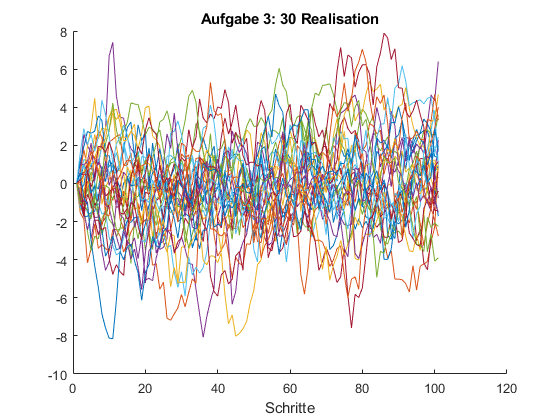
\includegraphics[width=0.9\textwidth]{images/30realisation} 
	\caption{30 Realisationen} 
	\label{fig:30real}
\end{figure}
Varianz: \ref{fig:var3}
\begin{figure}[htbp]
	\centering
	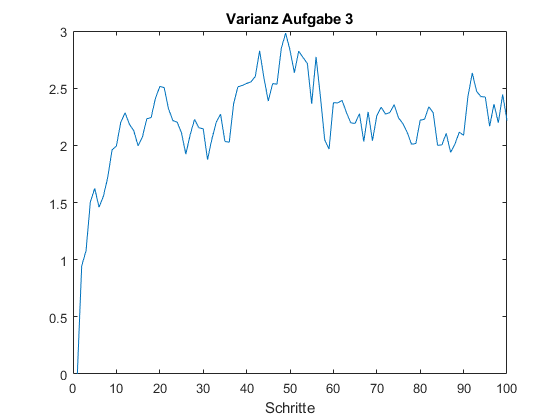
\includegraphics[width=0.8\textwidth]{images/var3} 
	\caption{Standardabweichung} 
	\label{fig:var3}
\end{figure}\\
Wenn es gibt keine Rauschen, bleiben $x = 0$ konstant, bei aller Realisationen sind $x$ zwischen 8 und -8. Deshalb schwingt Standardabweichung.
\clearpage
\section{Aufgabe 4}
\begin{gather}
	\bm{F} = \begin{bmatrix}
	0 & 1 \\
	0 & 0 
	\end{bmatrix} \Longrightarrow \Phi = \begin{bmatrix}
	1 & 1 \\
	0 & 1
	\end{bmatrix}
\end{gather}
$w$ nimmt man aus der Datei \textit{randoma4.txt}. 
Die Mittelwert sind aus den 50 Realisationen bei 20 Schritte: 
\begin{table}[htpb] \centering
	\begin{tabular}{cccc}
		Schritt & Mittelwert & Schritt & Mittelwert \\
		1       & 0          & 11      & -1,6929    \\
		2       & -0,0052    & 12      & -2,1167    \\
		3       & -0,0213    & 13      & -2,5194    \\
		4       & -0,0213    & 14      & -2,9730    \\
		5       & -0,1213    & 15      & -3,3244    \\
		6       & -0,2711    & 16      & -3,6583    \\
		7       & -0,6755    & 17      & -3,9089    \\
		8       & -0,8172    & 18      & -4,1349    \\
		9       & -1,0429    & 19      & -4,2768    \\
		10      & -0,3382    & 20      & -4,3405   
	\end{tabular}
	\caption{Mittelwerte}
	\label{tab:mittelwert}
\end{table}\\
graphische Darstellung der Mittelwerte \ref{fig:mittel4}
\begin{figure}[htbp]
	\centering
	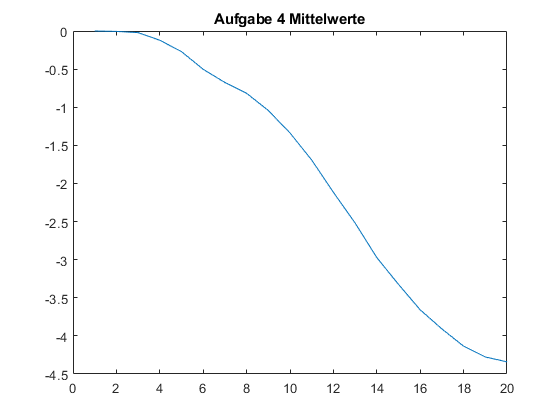
\includegraphics[width=0.8\textwidth]{images/4_mittelwerte} 
	\caption{Mittelwert von 30 Realsation} 
	\label{fig:mittel4}
\end{figure}\\
\begin{figure}[htbp]
	\centering
	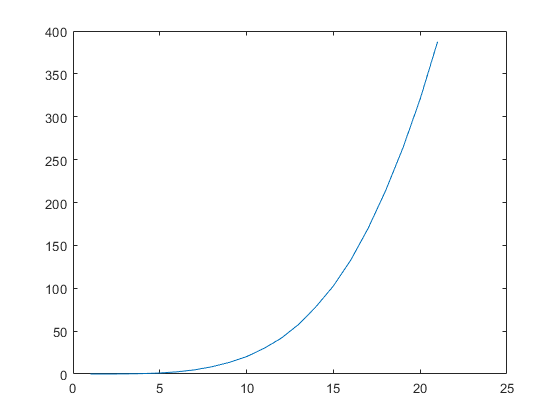
\includegraphics[width=0.8\textwidth]{images/var4} 
	\caption{Standardabweichung von 30 Realsation in jedem Schritt} 
	\label{fig:var4}
\end{figure}\\
Die Geschwindigkeit und Beschleunigung bei $t=0$ ist 0. $x$ soll 0 bleiben ohne Rauschen, aber die Mittelwerte weicht von 0 ab \ref{fig:mittel4}. Deshalb ist Standardabweichung immer größer \ref{fig:var4}.
\clearpage
\section{Aufgabe 5}
für $\Delta t = 1$\\\\
Gegebene Werte: $w_0 = 0,1$, $b^2 = 2\sqrt{2}w_0^3$
\begin{gather}
	\bm{F} = \begin{bmatrix}
	0 & 1 \\
	-w_0^2 & -\sqrt{2}w_0
	\end{bmatrix} \\
	\bm{\Phi} = \bm{I} + \bm{F} \Delta t + \frac{\bm{F}^2 \Delta t^2}{2!} + \cdots = \begin{bmatrix}
	0,9952 & 0,9310 \\
	-0,0093 & 0,8636 
	\end{bmatrix}\\
	 \bm{G} = \begin{bmatrix}
	 0\\
	 b
	 \end{bmatrix} = \begin{bmatrix}
	 0 \\
	 0,0532
	 \end{bmatrix}\\
	 \bm{Q} = \bm{\Phi} \bm{G} \bm{\Phi}^T \bm{G}^T = \begin{bmatrix}
	 2,45 & 2,27 \\
	 2,27 & 2,11
	 \end{bmatrix} \cdot 10^{-3}
\end{gather}